\documentclass[12pt]{article}
\usepackage{graphicx}

\oddsidemargin  -0.5 cm
\evensidemargin 0.0 cm
\textwidth      6.5in
\headheight     0.0in
\topmargin      -1 cm
\textheight=9in

\renewcommand{\arraystretch}{1.25}

\title{Alignment of the CMS Muon System \\ with the HIP Algorithm}
\author{Jim Pivarski, Karoly Banicz, Alexey Kamenev, Alexei Safonov}

\begin{document}
\maketitle

\section{Introduction}

The positions and orientations of CMS muon chambers must be well
understood for accurate measurements of muon momentum, especially for
muon tracks with energies on the order of
1~TeV~\cite{alignment_needed_for_tev}.  In addition to monitoring
these parameters with a dedicated apparatus~\cite{hardware_alignment},
we will also measure the alignment using tracks identified by the
chambers themselves using the HIP algorithm.  This track-based
alignment has several advantages, the most important being that tracks
reveal the positions of the sensitive elements directly, rather than
through the structure that supports them, and the precision on each
degree of freedom is proportional to that which is needed for track
reconstruction.

The fundamental difficulty in aligning any detector with the tracks it
observes is that the process of fitting tracks depends on the assumed
position of the detector.  One immediate consequence of this circular
dependence is that the global position of the whole detector can never
be determined with tracks alone.  Therefore, our emphasis will be on
relative alignments of one system to another, usually the chambers of
the muon system (barrel and endcap) relative to the silicon tracker,
but also muon chambers relative to one another.

\subsection{The HIP algorithm}

The HIP algorithm (Hits and Impact Points,~\cite{hip_algorithm})
addresses the interdependence of track fitting with alignment by
alternating between the two in an iterative approach.  The alignment
step is very simple: chambers are moved in such a way as to make the
weighted mean of their residuals distribution zero before refitting.
(A residual is the difference between the track's extrapolation to the
detector surface, called the impact point, and the measured hit.)

To illustrate this method, let's consider the algorithm in a
one-dimensional case.  At each iteration, the correction to the
$x$ position of the chamber is equal to the weighted mean of the $x$
residual distribution, negated.
\begin{equation}
\mbox{Alignment correction} = -\frac{b}{A} \pm \frac{1}{A} \mbox{ with } A =
\sum_{\mbox{\scriptsize all hits}} \frac{1}{{\sigma_r}^2}
\mbox{ and } b = \sum_{\mbox{\scriptsize all hits}} \frac{r}{{\sigma_r}^2} \mbox{,}
\label{weighted_mean}
\end{equation}
where $r$ is the residual (track minus hit) and $\sigma_r$
is its uncertainty, for each hit.

In general, each hit in the real detector measures one or two
dimensions in its sensitive plane (residuals $\vec{r}$ = $r_x$ and
$r_y$ with covariance matrix ${\sigma_r}^2$) which are transformed to the
(at most) six-dimensional space of local alignment corrections
$\vec{q}$ = $x$, $y$, $z$, $\phi_x$, $\phi_y$, and $\phi_z$ through an
(at most) 6$\times$2 Jacobian matrix $(\partial q/\partial r)$.  (We
can fix degrees of freedom that are not well determined, reducing the
dimensionality of the problem.)  The alignment corrections still look
like a weighted mean:
\begin{equation}
\mbox{Alignment corrections} = -{\bf A}^{-1} \cdot \vec{b} \ \pm\  {\bf A}^{-1}
\label{alignment_corrections1}
\end{equation}
where
\begin{equation}
{\bf A} = \sum_{\mbox{\scriptsize all hits}} \,
  \left(\frac{\partial q}{\partial r}\right) \,
  \left({\sigma_r}^2\right)^{-1} \,
  \left(\frac{\partial q}{\partial r}\right)^T
\end{equation}
and
\begin{equation}
\vec{b} = \sum_{\mbox{\scriptsize all hits}} \,
  \left(\frac{\partial q}{\partial r}\right) \,
  \left({\sigma_r}^2\right)^{-1} \,
  \vec{r} \mbox{.}
\label{alignment_corrections2}
\end{equation}
Since the matrix inversions are at most 6$\times$6, most
of the computational effort in the HIP algorithm is spent re-fitting
tracks and producing updated residuals distributions between
iterations.

\subsection{The geometry of the muon system}

The muon system is composed of a barrel of drift tube chambers and two
endcaps of cathode strip chambers surrounding all other CMS detectors
(see Figure~\ref{muon_system_labeled}).

\begin{figure}
\begin{center}
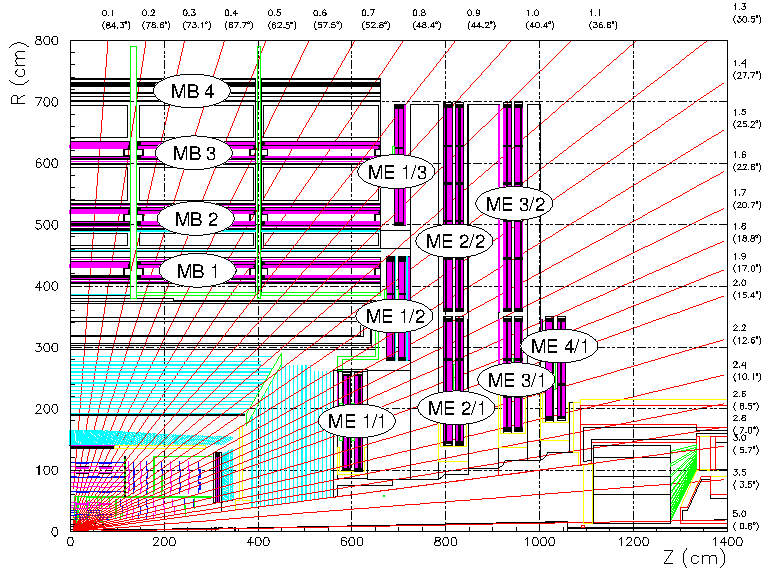
\includegraphics[width=0.75\linewidth]{intro/muon_system_labeled.pdf}
\end{center}

\caption{\label{muon_system_labeled} A quarter-view of CMS,
  highlighting the muon barrel (MB) and endcap (ME) stations.}
\end{figure}

A drift tube is an anode wire in a cylindrical, gas-filled tube, held
at high voltage with respect to the outer surface of the tube.  It
measures the distance of closest approach of a charged track to the
wire through the time needed for electrons to drift from gas atoms,
ionized by the track's passage, to the wire \cite{drift_tubes}.

Drift tube chambers (DTs) are rectangular sandwiches of 8--12 layers
of drift tubes.  Each layer measures the intersection of the track
with the layer plane in one dimension: $x$ in local chamber
coordinates for the first four layers (superlayer 1) and the last four
layers (superlayer 2 or 3).  Chambers with 12 layers (all but MB 4:
see Figure~\ref{muon_system_labeled}) have a third superlayer in the
middle that measures $y$ in local chamber coordinates, being rotated a
90$^\circ$ angle with respect to superlayers 1 and 3.  In global CMS
coordinates, the DTs' local $x$ corresponds roughly with $r\phi$, the
polar angle around the beamline, and local $y$ corresponds exactly with
global $z$, the direction along the beamline.  The layers are stacked
in local $z$.

There are 250 DTs: 4 stations in global $r$ times 5 wheels in global
$z$ times 12--14 sectors in global $\phi$.  (Only MB 4 has 14
sectors.)

A cathode strip is a band of conducting material painted on a layer
plane, measuring the intersection of a track through that plane by
comparing the charges collected on neighboring strips.  In the cathode
strip chambers (CSCs), 6 trapezoidal layers of cathode planes
alternate with layers of anode wires.  The strips measure the track
intersection point along a dimension which is nearly collinear with
local $x$: ``nearly'' because the strips fan from the narrow end of
the trapezoid to the wide end, and only the central strip measures $x$
exactly (see Figure~\ref{csc_chamber}).  The wires measure the same
intersection point in the local $y$ direction.  Just as for the DTs,
local $x$ corresponds roughly with $r\phi$ in the global CMS
coordinate system, but for CSCs, local $y$ corresponds roughly with
global $r$.  The CSC layers are also stacked in local $z$, but in
decreasing order (layer 1 is ``above'' layer 6 in $z$).

\begin{figure}
\begin{center}
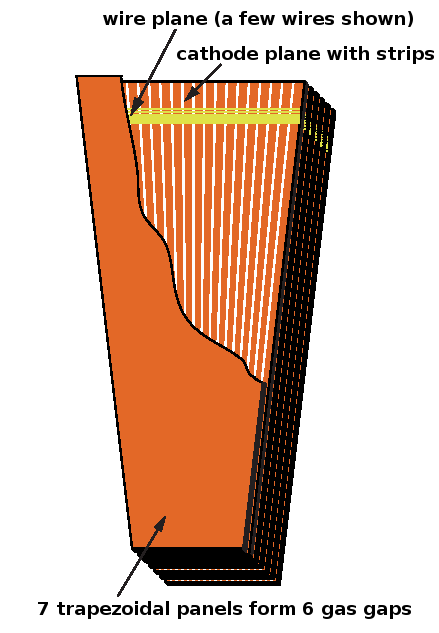
\includegraphics[width=0.3\linewidth]{intro/csc_chamber.png}
\end{center}

\caption{\label{csc_chamber} A CSC chamber: cathode strips measure the
  local $x$ direction (global $r\phi$) and wire groups measure the
  local $y$ direction (global $r$).}
\end{figure}

For alignment purposes, there are 540 CSC chambers, not all of which
are physically distinct.  Chambers in ME 1/1 (see
Figure~\ref{muon_system_labeled}) have a unique geometry: they are
doubled (12 active layers) in such a way that each may be treated as two
chambers~\cite{doubling_up_me11}.  In the geometry description used by
track reconstruction, half of each double-chamber is said to belong to
a new station, ME 1/4.  We will use the same convention.

The intrinsic resolution of a DT hit ($x$ or $y$) is approximately
300~$\mu$m~\cite{intrinsic_dt_resolution}.  The intrinsic resolution
of a CSC hit can be as small as $\sim$200~$\mu$m in local $x$ if the
track intersection is between strips, $\sim$??~$\mu$m otherwise.
(Strips are staggered from one layer to the next to guarantee that
about half of the hits will have optimum precision in $x$.)  Local $y$
resolution is about 1~cm for CSCs because groups of neighboring wires
are ganged together to make read-out
feasible~\cite{intrinsic_csc_resolution}.  Since the hit uncertainties
loosely distinguish between different types of hits, error propagation
in Equation~\ref{alignment_corrections2} is crucial: we must align to
the weighted mean, rather than the unweighted mean.

The goal of track-based alignment is to measure the positions of each
chamber with a better precision than the intrinsic resolution.  We
will treat each chamber as a rigid body; layers and superlayers have
been firmly locked in place.  However, the positions of internal
elements may differ from their design geometry, so we will use
measurements of DT layers and superlayers provided by the DT alignment
group~\cite{dt_alignment_group} and CSC layers from the CSC alignment
group~\cite{csc_alignment_group}.  Additionally, we will refine the
CSC layer determination with a special track-based alignment run,
described below.

DT and CSC chambers are allowed to slide and rotate when the 4~T
magnetic field turns on and off (several millimeters in the CSC case),
to protect their internal structure from stresses from the enormous
force of the field~\cite{slide_in_field}.  Therefore, chamber
positions are always treated as floating parameters.  Additionally,
the DT chambers are mounted on 5 free-standing wheels and the CSC
chambers are mounted on 4 free-standing disks for each endcap (total
of 8).  These can slide open and closed (on air and grease pads) to
provide access to CMS's inner detectors.  As a result, the wheels and
disks are a source of correlated alignment error, observed to be
as large as 7~mm.  To avoid individually aligning all chambers on a
wheel or disk by what is really a combined motion (for instance, 7~mm
to the left), we will first align the wheels and disks as units,
followed by the chambers.

\section{General configuration and organization of studies}

\subsection{Nominal alignment procedure}

In this section, we describe the nominal procedure that is used as a
standard of comparison for systematics studies.  The nominal procedure
is not necessarily the best procedure: in the course of our studies,
we find improvements on our initial best guess and present the optimal
procedure at the end of each section as a recommendation.

The nominal procedure is conducted in two parts: first we align the
barrel wheels and endcap disks relative to the CMS silicon tracker,
then we align the individual chambers, also using the silicon tracker
as a reference.  We studied relative alignment of muon chambers
without an external reference, but present that in a later section.
We also discuss procedures for CSC layer alignment (the third
alignment step) in its own section.

Nominal alignment requires a source of high-$p_T$ muons from the
14~TeV $p$-$p$ collision vertex.  We assume that the rate of this
source is the rate of $W\to\mu\nu$ and $Z\to\mu\mu$ muons (effectively
6.6~nb and 0.5~nb, respectively, when branching fractions and
acceptance are included) in collisions at $2\times
10^{32}$~/cm$^2$/s luminosity (0.2~nb$^{-1}$/s).  In our simulations,
we only generate $Z\to\mu\mu$ muons, and extrapolate to equal numbers
of muon tracks.  In a later section, we explore the effects of
aligning with inclusively-selected muons and larger samples of
lower-$p_T$ muons.  We also postpone discussions of alignments with
other sources, such as beam-halo muons from the accelerator, and
the results from cosmic ray alignments to a later section.

\subsection{Initial conditions: the misalignment scenario}

To study our alignment procedure in Monte Carlo, we must begin with a
realistically misaligned detector.  Wheels, disks, chambers, and CSC
layers are misaligned once by random translations and rotations at the
beginning of the alignment process, drawn from Gaussian distributions.
Subdetectors, such as chambers on a wheel or disk, or layers in a
chamber, are displaced relative to the displaced superstructure,
thereby introducing correlations among subdetectors on the same
superstructure.  The standard deviations of the Gaussians used to
generate misalignments are given in Table~\ref{misalignments}.  Most
values are conservative estimates, the exception being the magnitudes
for CSC layers, taken from measurements with cosmic
rays~\cite{karoly_layer_misalignments}.  These misalignments are all
larger than the 10~pb$^{-1}$ projection (Muon10InvPbScenario) used for
misalignment studies in physics analyses.

\begin{figure}
\begin{center}
\begin{tabular}{l c c c c c c}
\hline\hline Component & $x$ (cm) & $y$ (cm) & $z$ (cm) & $\phi_x$ (mrad) & $\phi_y$ (mrad) & $\phi_z$ (mrad) \\\hline
Barrel wheels & 1 & 1 & 1 & 1 & 1 & 1 \\
DT chambers & 0.3 & 0.3 & 0.3 & 1 & 1 & 1 \\\hline
Endcap disks & 1 & 1 & 1 & 1 & 1 & 1 \\
CSC chambers & 0.3 & 0.3 & 0.3 & 1 & 1 & 1 \\
CSC layers & 0.0190 & 0.0340 & 0 & 0 & 0 & 0.040 \\\hline\hline
\end{tabular}
\end{center}

\caption{\label{misalignments} Standard deviations of the Gaussians
used to generate misalignments as a starting point for alignment
studies.  Values for CSC layers come from measurements of a subset
with cosmic rays; the rest are conservative estimates.}
\end{figure}

We align the muon system relative to the silicon tracker by
extrapolating tracks from the tracker to the muon system.  This makes
the muon alignment resolution dependent on the tracker misalignment, a
dependence which we will quantify.  For the nominal procedure, we use
the short-term tracker misalignment scenario intended for misalignment
studies in physics analyses (TrackerShortTermScenario).

\subsection{Track refitting procedure}

At each iteration of the HIP algorithm, tracks selected for alignment
are refit (from the outermost hits inward) under the current alignment
conditions.  This allows misalignments and alignment corrections to be
propagated into the residual distributions, as residuals are
calculated from the tracks' intersections with the assumed positions of
the detector planes.  We also have the opportunity to reweight the
hits used in the track fit through the detectors' alignment parameter
errors (APEs).  The inverse weight of each hit ($\sigma_r$ in
Equation~\ref{weighted_mean}) is given by
\begin{equation}
{\sigma_r}^2 = {\sigma_{\mbox{\scriptsize track}}}^2 +
{\sigma_{\mbox{\scriptsize hit}}}^2 + {\sigma_{\mbox{\scriptsize APE}}}^2
\label{hit_uncertainty}
\end{equation}
where $\sigma_{\mbox{\scriptsize track}}$ is the uncertainty in the
track projection, $\sigma_{\mbox{\scriptsize hit}}$ is the intrinsic
hit uncertainty, and $\sigma_{\mbox{\scriptsize APE}}$ is the
alignment parameter error.

To decouple track-fitting from alignment, we severely deweight the
hits in the muon system by giving them each a
$\sigma_{\mbox{\scriptsize APE}}$ of 10~cm.  Track fits are thus
dominated by the silicon tracker, but muon chamber residuals are still
calculated and track fits are still sensitive to large kinks from
multiple scattering.  With this technique, alignment reaches its final
accuracy in one iteration, because the fitted positions of tracks are
largely undisturbed by moving the muon chambers.

It is important to verify that the optimum placement of muon chambers
is not a function of $\sigma_{\mbox{\scriptsize APE}}$.  For instance,
we might imagine that one detector geometry optimizes residual
distributions when muon hits are insignificant in the track-fit, and
another geometry optimizes residual distributions in standard track
reconstruction.  We check for this by decreasing
$\sigma_{\mbox{\scriptsize APE}}$ from 10~cm to a negligible value,
superexponentially with iteration number (according to
\begin{equation}
\sigma_{\mbox{\scriptsize APE}} = (10\mbox{ cm}) \, \exp\left(-\frac{i^3}{10}\right)
\end{equation}
where $i$ is the number of completed iterations).
After three iterations, $\sigma_{\mbox{\scriptsize APE}}$ falls
below $\sigma_{\mbox{\scriptsize hit}}$ and track reconstruction
becomes equivalent to the standard offline reconstruction algorithm
(see Figure~\ref{residuals_by_iteration}).  As we will later see,
aligned positions after the fourth iteration are the same as aligned
positions in the first three iterations, validating our procedure.

\begin{figure}
\begin{center}
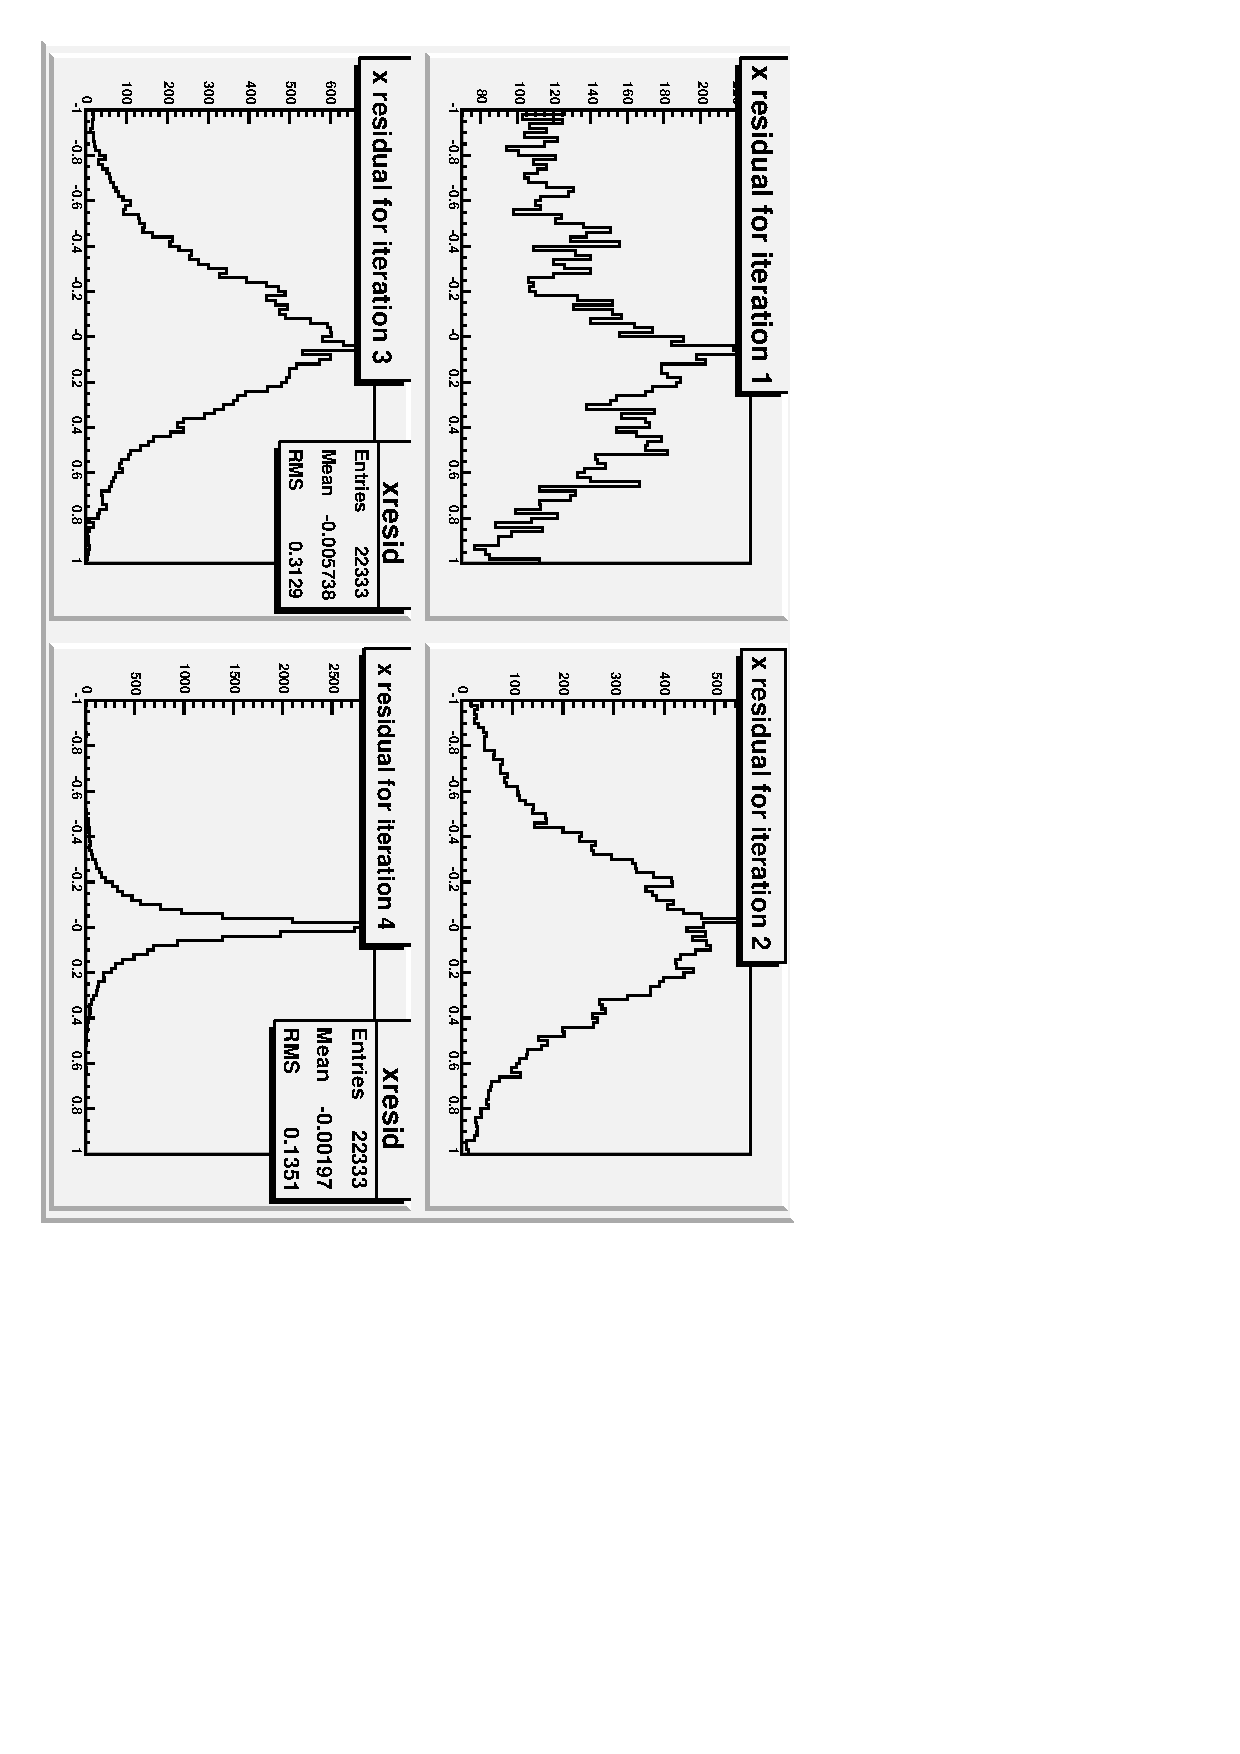
\includegraphics[height=0.75\linewidth, angle=90]{disk_alignment/residuals_by_iteration.pdf}
\end{center}

\caption{\label{residuals_by_iteration} Residual distributions ({\it not}
  weighted by $1/{\sigma_r}^2$) in the first four iterations of a wheel/disk
  alignment, illustrating the transition from
  $\sigma_{\mbox{\scriptsize APE}}$-dominated track fits in the first
  three iterations to standard reconstruction from iteration 4
  onward.}
\end{figure}

\subsection{Software framework}

CommonAlignment, AlignmentProducer,
HIPAlignmentAlgorithm~\cite{alignment_software};
CommonAlignmentMonitor, AlignmentMonitorMuonHIP,
muonHIP.py~\cite{my_alignment_software}

\section{Wheel and disk alignment}

In a wheel/disk alignment, the alignment parameters are all expressed
in global coordinates: $x$ is parallel to the floor in the CMS cavern,
$y$ points upward, and $z$ is along the beamline.  The most sensitive
parameter is $\phi_z$, rotation around the beamline, since this
corresponds to the most sensitive measurement dimension in all
chambers.  It is also the most relevant for accurately reconstructing
muon $p_T$.

The second-most sensitive parameters are $x$ and $y$.  The $x$
alignment is dominated by the chambers on the top and bottom of each
wheel/disk, and $y$ is dominated by chambers on the sides because the
local $x$ measurements of each chamber are better than the local $y$
measurements.  Wheels are directly sensitive to their $z$ positions,
but disks are only sensitive through imprecise local $y$ measurements
times $\cot\theta$, where $\theta$ is the azimuthal angle of the
tracks with respect to the beamline.  In the nominal wheel/disk
alignment, only $x$, $y$, and $\phi_z$ are allowed to float.

\subsection{Nominal results and consistency checks}

The left-hand plot of Figure~\ref{phiz_conv} presents the result of a
typical wheel/disk alignment: $\phi_z$~for each of the 13 wheels and
disks starts with an $\mathcal{O}(\mbox{1 mrad})$ misalignment and is
brought within $\mathcal{O}(\mbox{0.2 mrad})$ of the correct alignment in
the first iteration.  The geometry doesn't change significantly
between iterations 3 and 4, so the alignment is not dependent on
$\sigma_{\mbox{\scriptsize APE}}$.

\begin{figure}
\begin{center}
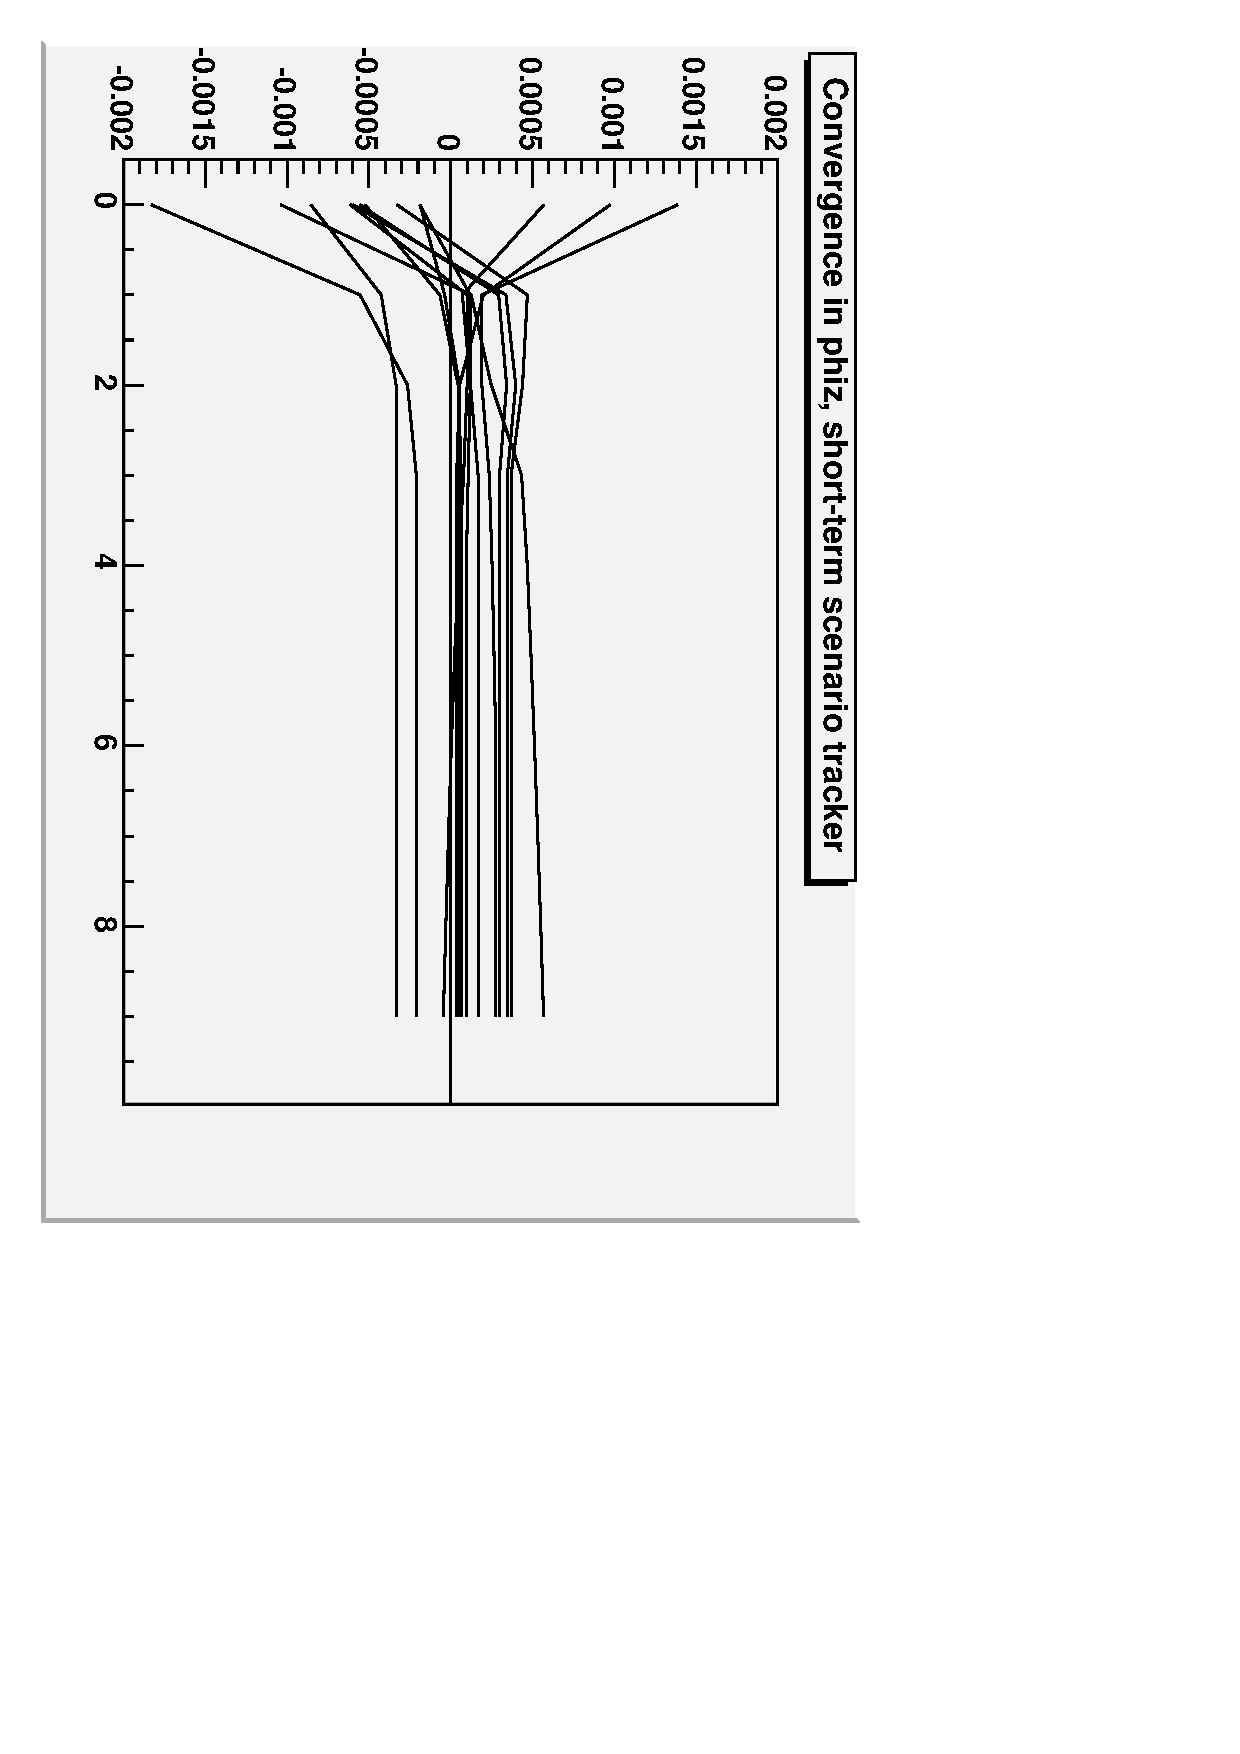
\includegraphics[height=0.45\linewidth, angle=90]{disk_alignment/phiz_conv_nominal.pdf}
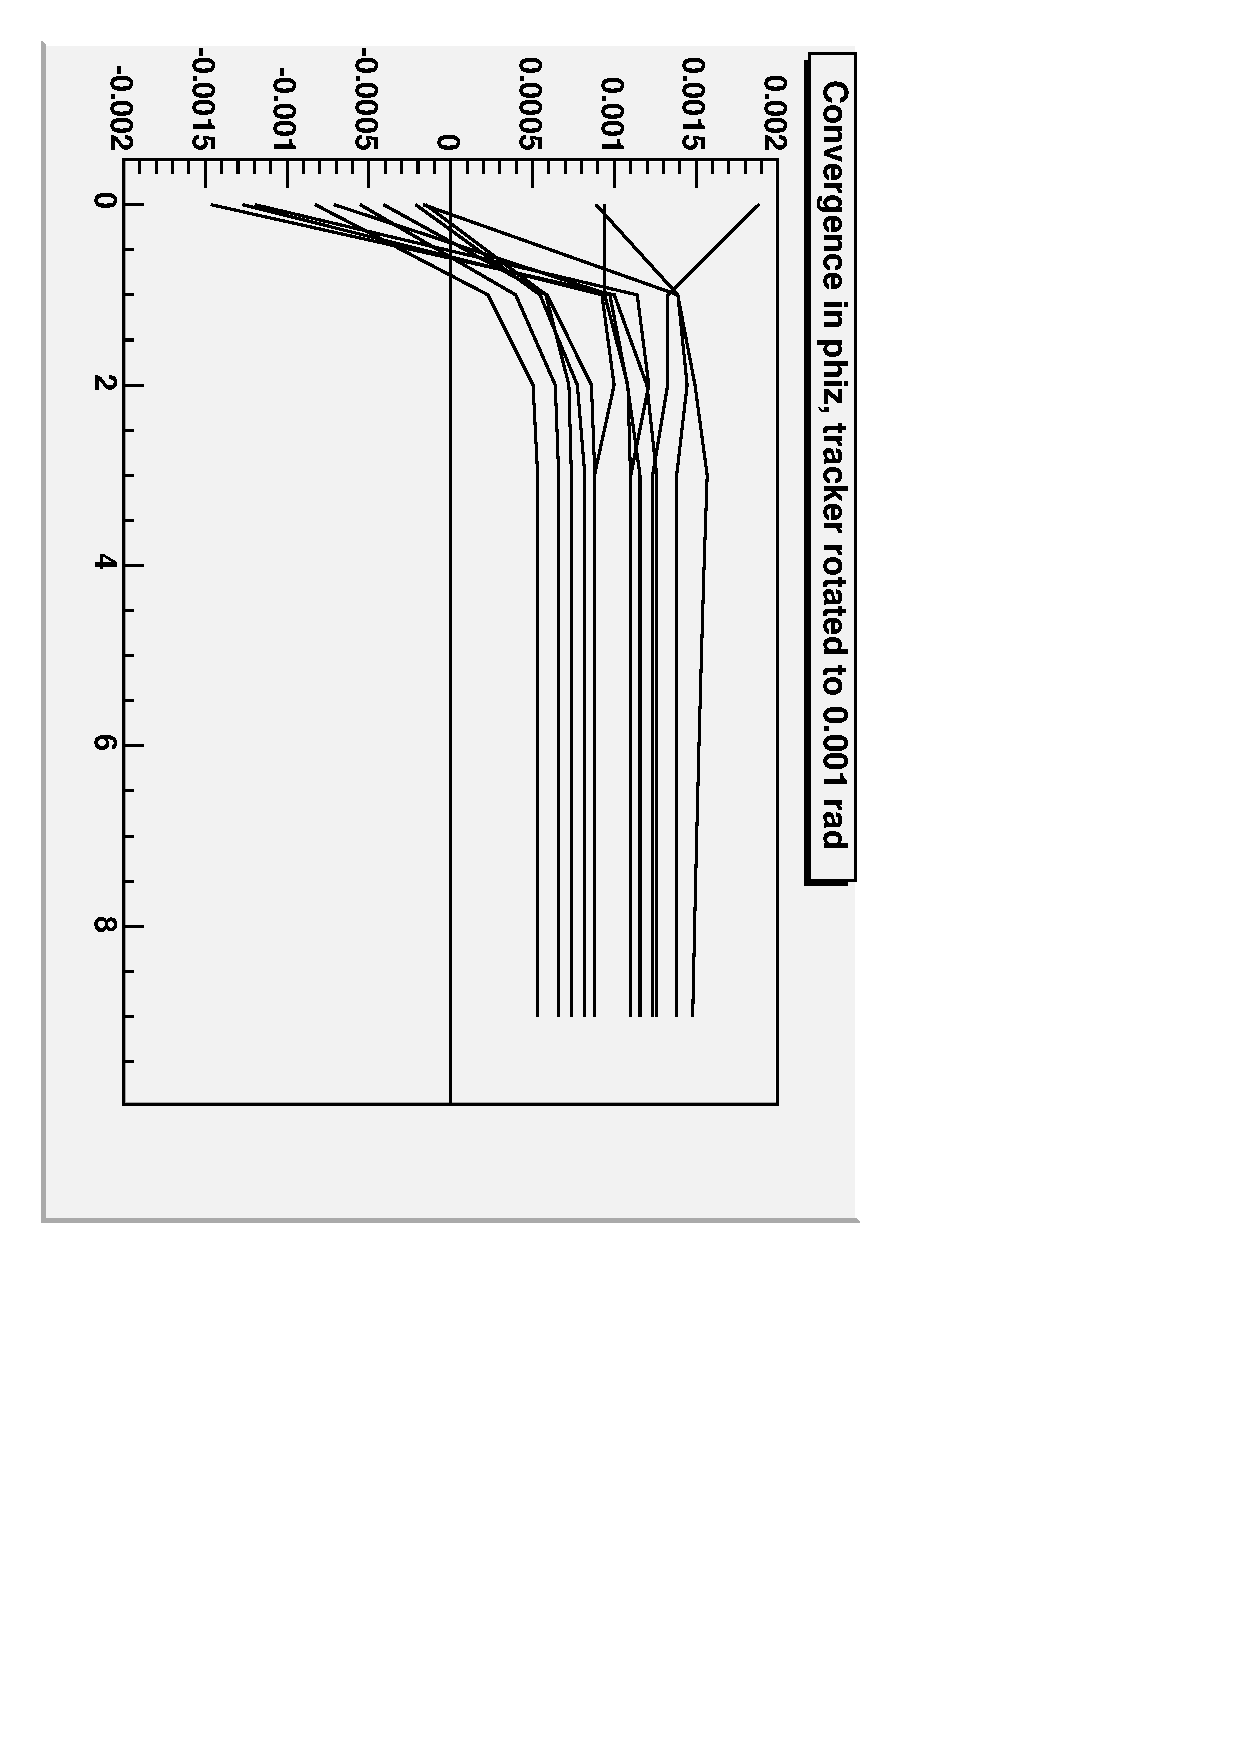
\includegraphics[height=0.45\linewidth, angle=90]{disk_alignment/phiz_conv_barrel_roll.pdf}
\end{center}

\caption{\label{phiz_conv} Left: convergence of $\phi_z$ as a function
  of iteration.  Right: a simulation with the tracker rotated 1~mrad.}
\end{figure}

In this simulation and most alignment simulations presented in this
note, the correct geometry that the alignment procedure should tend
toward is the ideal, or design geometry of the detector.  The same is
not necessarily true in real alignments with data.  To be sure that
the alignment procedure is not artificially tending toward the ideal
geometry, we rotated the tracker by 1~mrad, making the correct
geometry for each wheel and disk offset from ideal by a 1~mrad
$\phi_z$ rotation.  The result of this test is presented on the
right-hand side of Figure~\ref{phiz_conv}.  All of the wheels and
disks correctly tend toward 1~mrad instead of 0.

Thirteen wheels and disks is not a sufficiently large statistical
sample to determine the accuracy of the alignment procedure.  We
therefore repeat the exercise 10 times with different random starting
positions for all wheels, disks, chambers, and CSC layers in each
trial.  (The tracker alignment is the same in each trial.)  The
positions of 13$\times$10 aligned detectors are histogrammed, fit, and
tabulated in Figure~\ref{nominal_fits}.  Resolution in $x$ and $y$ is
1.31~$\pm$~0.12~mm and resolution in $\phi_z$ is 0.20~$\pm$~0.02~mrad.
We prefer this method for determining alignment resolutions over the
precision calculated by Equation~\ref{alignment_corrections1}, which
assumes correct track fits (no tracker misalignment) and depends
strongly on one's choice of $\sigma_{\mbox{\scriptsize APE}}$.

\begin{figure}
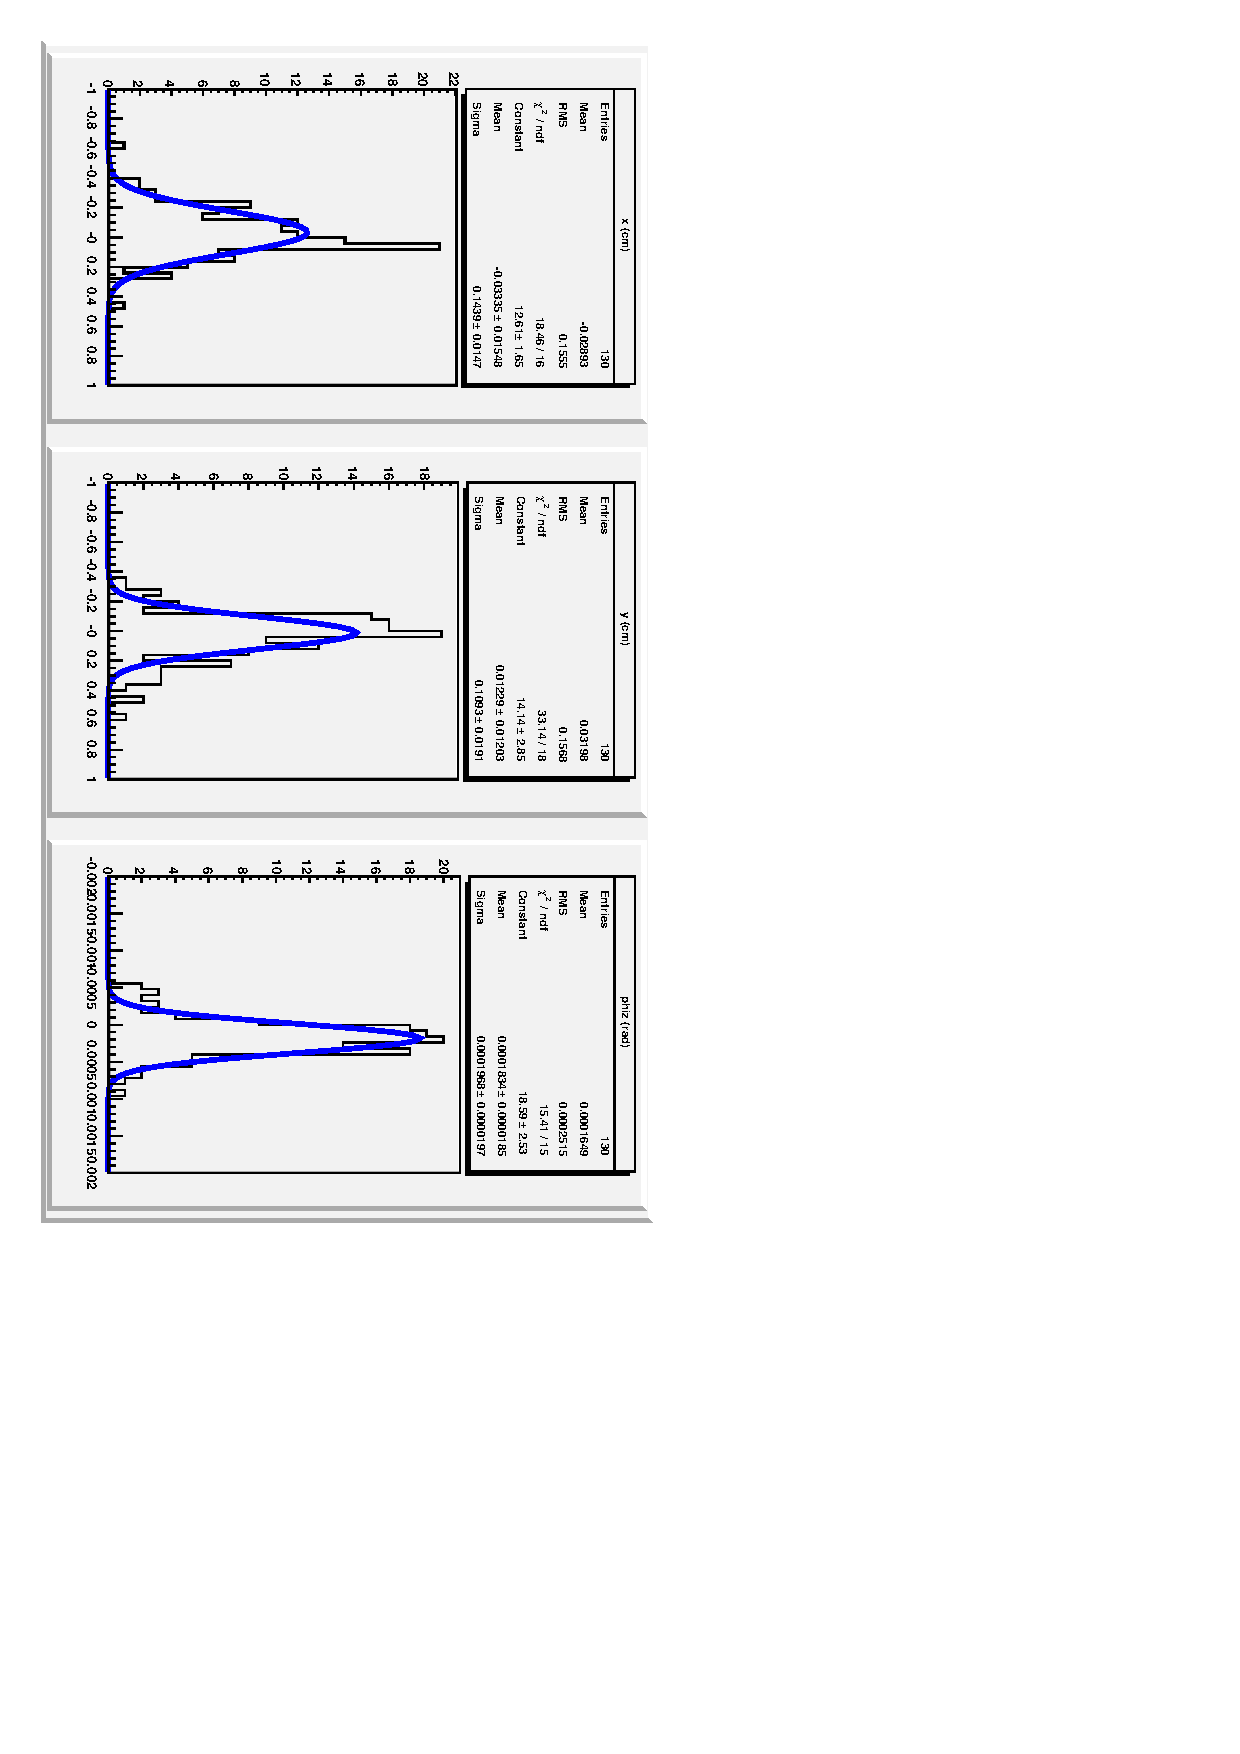
\includegraphics[height=\linewidth, angle=90]{disk_alignment/nominal_fits_color.pdf}

\caption{\label{nominal_fits} Aligned positions of all wheels and
  disks in 10 trials, randomizing the initial muon geometry with each
  trial.}
\end{figure}

\subsection{Dependence on tracker alignment}

Track-fits were provided by the silicon tracker, so it is natural to
ask how muon alignment resolution depends on tracker misalignment.  We
repeated the above analysis (muon alignment in 10 trials) for an ideal
tracker, twice the nominal short-term tracker misalignment, five times
and ten times the tracker misalignment.  This dependence is plotted in
black in Figure~\ref{vstracker}: the tracker must be 3.8~times more
misaligned than expected to degrade muon alignment by a factor of~2.

\begin{figure}
\begin{center}
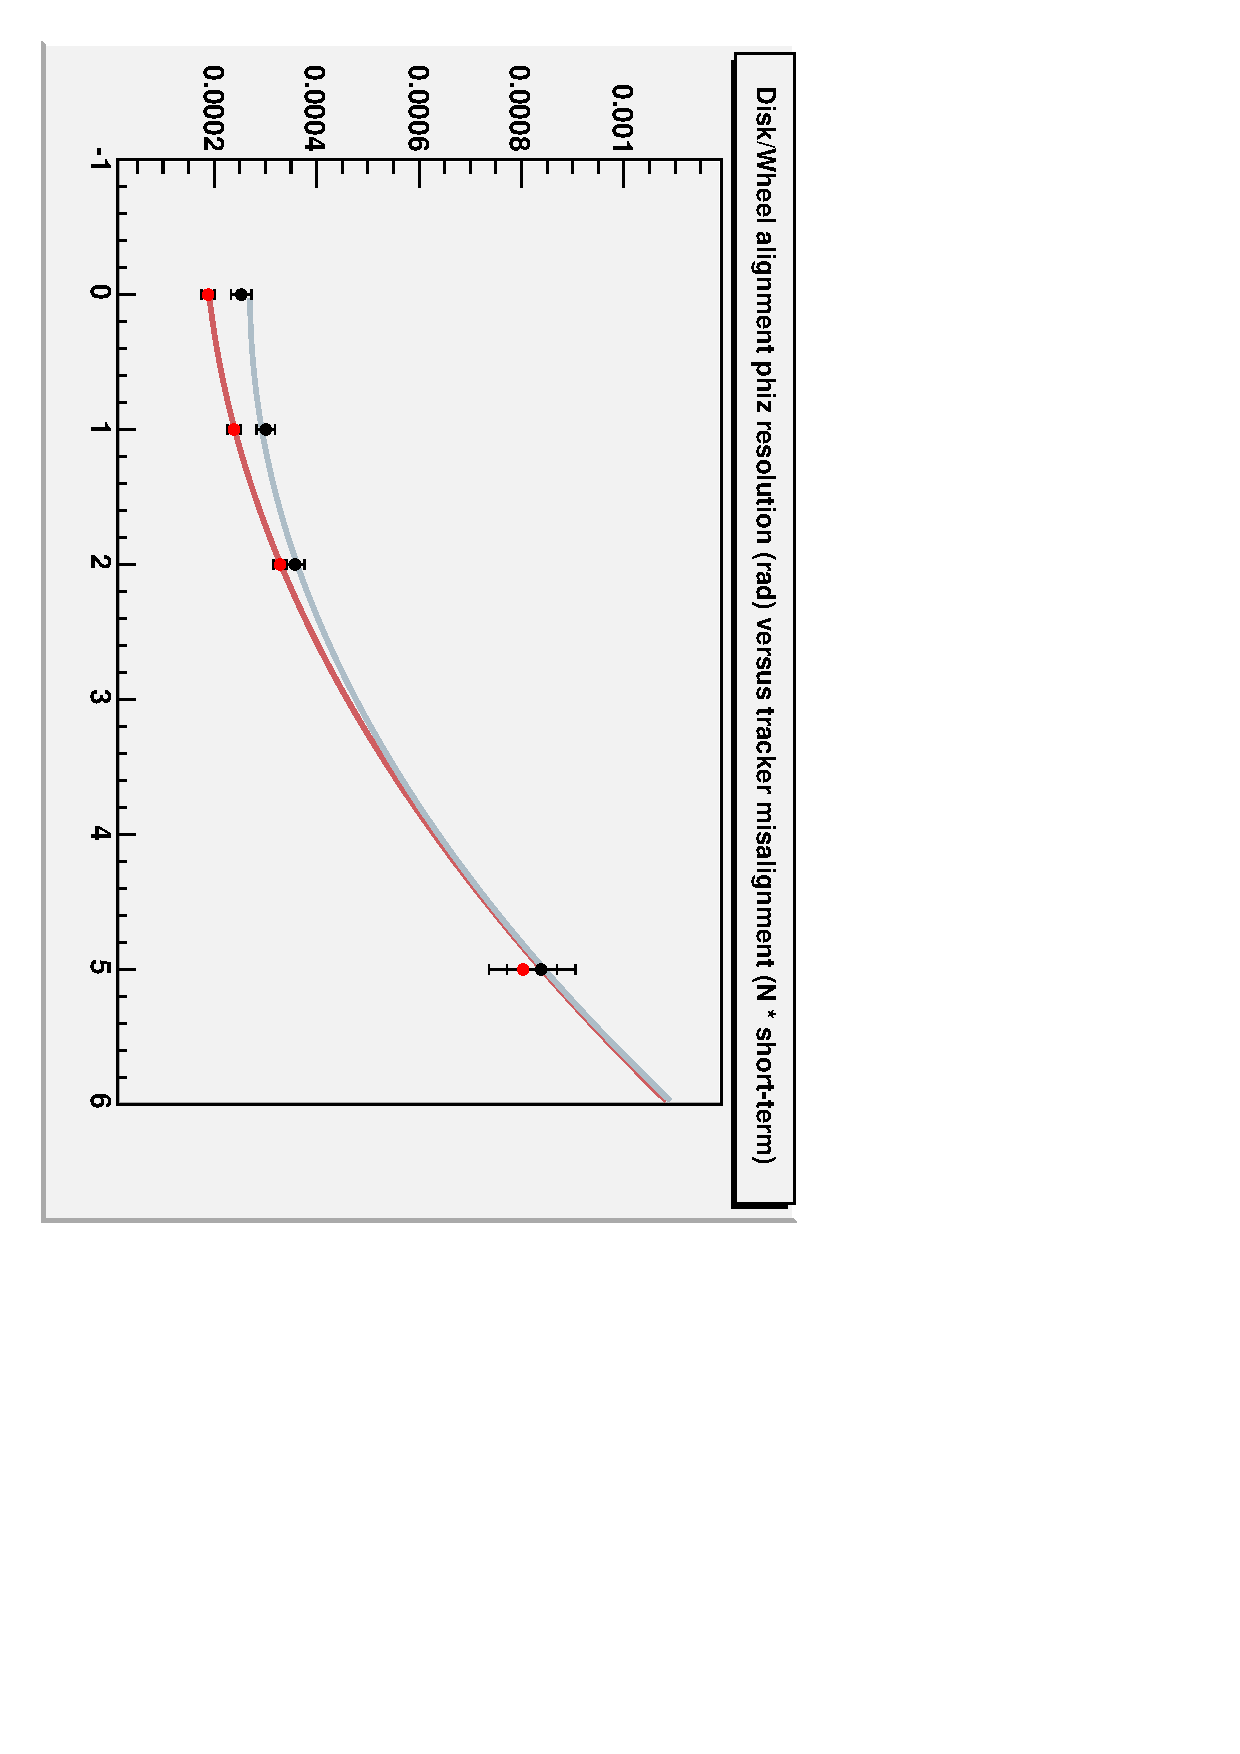
\includegraphics[height=0.75\linewidth, angle=90]{disk_alignment/vstracker2.pdf}
\end{center}

\caption{\label{vstracker} Dependence of muon alignment resolution on
  tracker misalignment, with (black) and without (red) internal
  misalignments (chambers and CSC layers).  The horizontal axis is a
  scale factor applied to tracker misalignment: 0 is an ideal tracker
  and 1 is the nominal short-term scenario.  The vertical axis is
  $\phi_z$ resolution.}
\end{figure}

One might conjecture that the variance in the aligned positions of
wheels and disks is dominated by internal misalignments: the
misaligned chamber positions that our wheel/disk procedure cannot
correct.  In that case, the accuracy of $\phi_z$ is a function of the
ratio of tracker misalignment to internal muon misalignment, and the
latter was chosen ad-hoc!  We therefore repeated the study with no
internal misalignments in the muon wheels and disks, and found that
the the curve is not greatly changed (plotted in red in
Figure~\ref{vstracker}).  Since the nominal internal misalignments
were conservative, the dependence of $\phi_z$ resolution on tracker
misalignment is somewhere between the red curve and the black curve
(closer to the black curve).

\subsection{Required integrated luminosity}

The wheel/disk alignment procedure requires very few muons to reach
its final accuracy.  Even with deweighted muon chambers, the
track-by-track residual distribution is 3~mm wide (see iteration 3 in
Figure~\ref{residuals_by_iteration}).  In principle, the wheel and
disk positions can reach a 1~mm accuracy with 10 tracks per detector,
though 10 tracks aren't guaranteed to be optimally distributed in
$\phi$.  We repeated the nominal procedure with 250, 500, 1000, and
2000 tracks, obtaining consistent results in each trial.  To improve
alignment beyond the millimeter scale, it is necessary to allow chambers to
float.

\subsection{Dependence on number of free parameters}

The nominal procedure, in which only $x$, $y$, and $\phi_z$ are
allowed to float in the alignment, is overly cautious.  Three out of
the eight superlayers in each barrel wheel measure the global $z$ of
hits directly, so we should at least let the $z$ positions of wheels
float.  Moreover, $\phi_x$ and $\phi_y$ orientation can be determined
from differences in $z$ position between the top and bottom chambers
(for $\phi_x$) and the left and right chambers (for $\phi_y$).  We
therefore get the best overall alignment by letting all 6 parameters
float for barrel wheels and only 3 parameters ($x$, $y$, and $\phi_z$)
for endcap disks.  Allowing more degrees of freedom for the disks
degrades their $z$, $\phi_x$, or $\phi_y$ alignment beyond the initial
configuration without aiding the alignment of any other parameters.

In Figure~\ref{alldt_3csc}, we present results for the 6-parameter
wheel, 3-parameter disk alignment.  The $x$ and $y$ resolutions are
0.71~$\pm$~0.04~mm, $z$ resolution is 0.89~$\pm$~0.11~mm, $\phi_x$ and
$\phi_y$ resolutions are 0.20~$\pm$~0.02~mrad, and $\phi_z$ resolution
is 0.11~$\pm$~0.01~mrad.

\begin{figure}
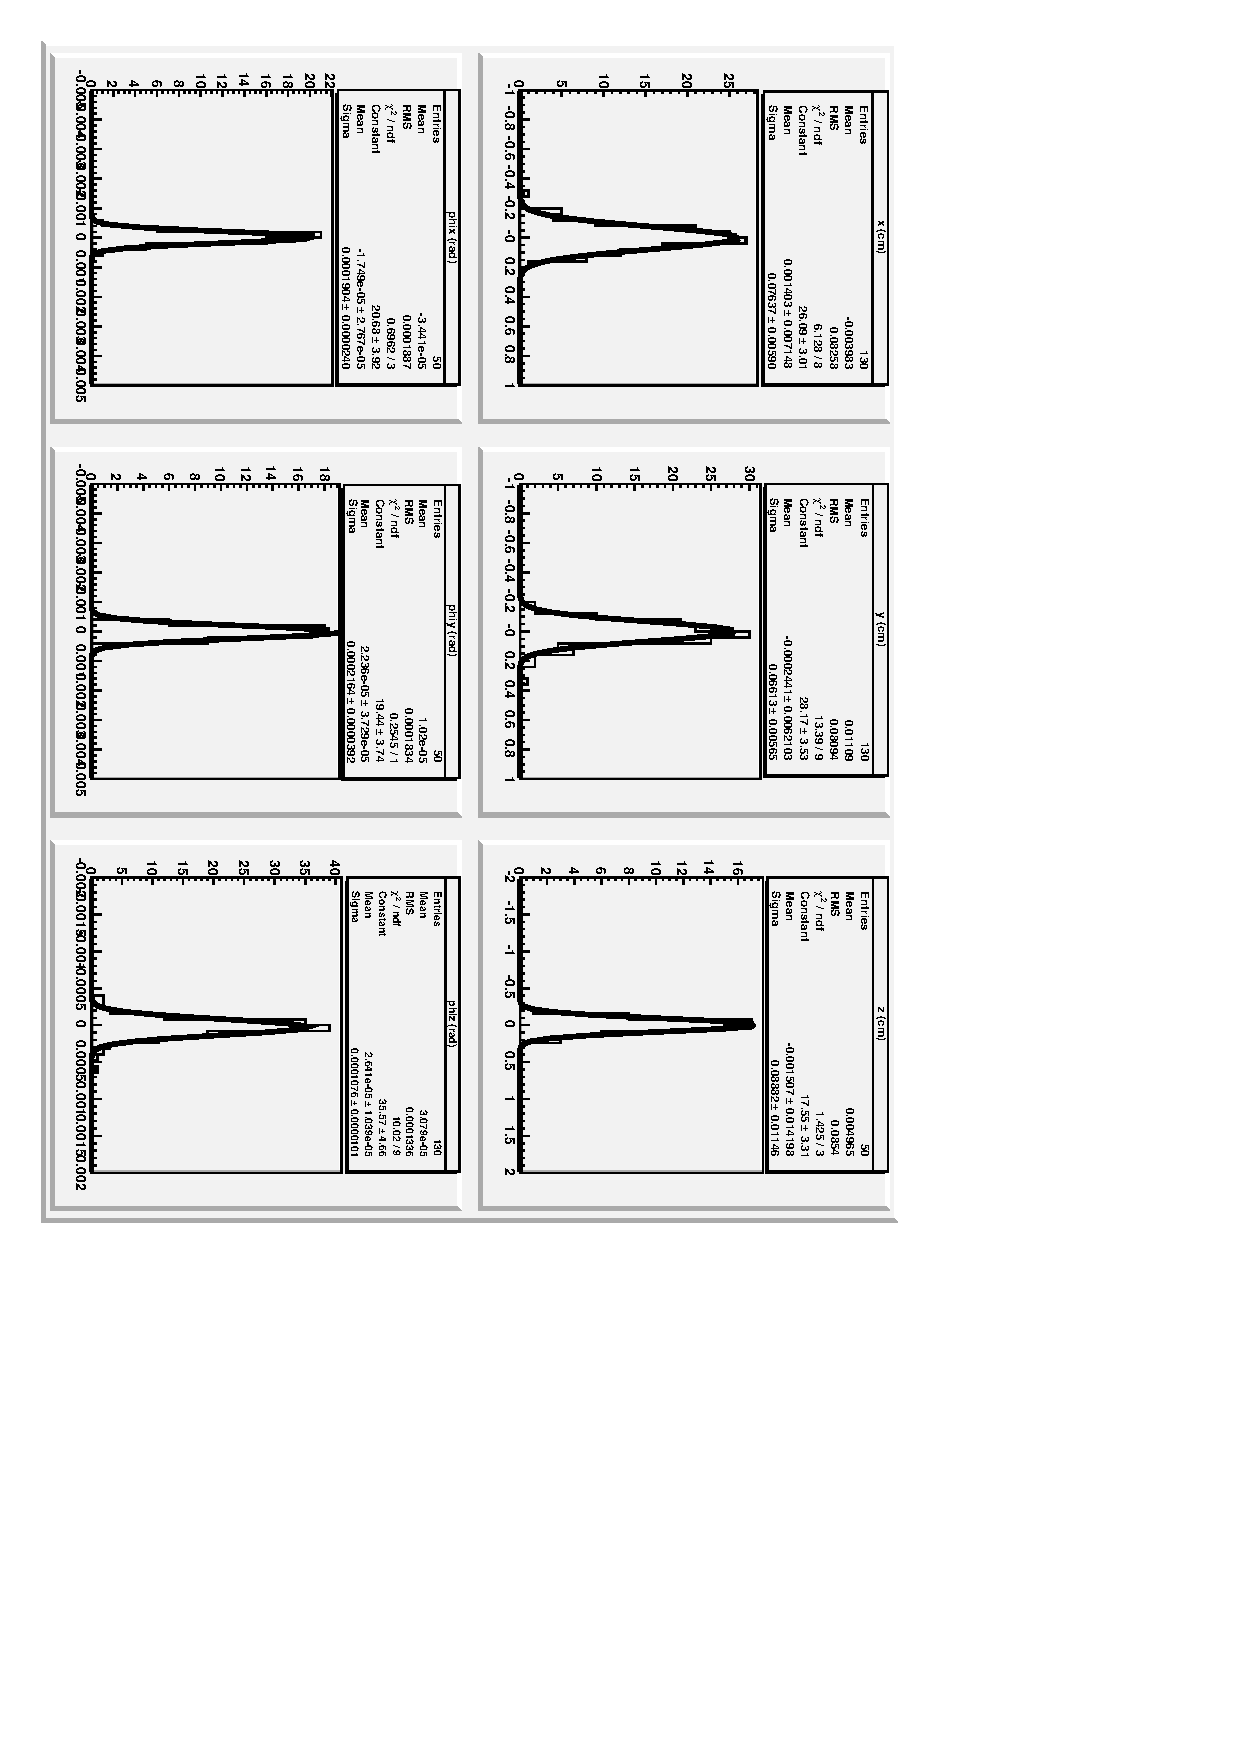
\includegraphics[height=\linewidth, angle=90]{disk_alignment/alldt_3csc.pdf}

\caption{\label{alldt_3csc} Optimal wheel/disk alignment, in which all
  6 parameters float for barrel wheels but only $x$, $y$, and $\phi_z$
  for endcap disks.  Note that 13 alignables $\times$ 10 trials are
  presented for $x$, $y$, and $\phi_z$, but only 5 alignables $\times$
  10 trials for $z$, $\phi_x$, and $\phi_y$.}
\end{figure}

\subsection{Recommended wheel/disk alignment configuration}

The 6-parameter wheel, 3-parameter disk alignment with at least 300
muons and 1 or 2 iterations is our recommended procedure for wheel and
disk alignment.  (The second iteration improves resolution by about
5\%.)  In early data, we will want to repeat some of the above tests
to make sure that data behaves as well as Monte Carlo.

\section{Chamber-by-chamber alignment}

\begin{figure}
\begin{center}
\begin{tabular}{p{0.31\linewidth} p{0.31\linewidth} p{0.31\linewidth}}
  \begin{minipage}{\linewidth}
    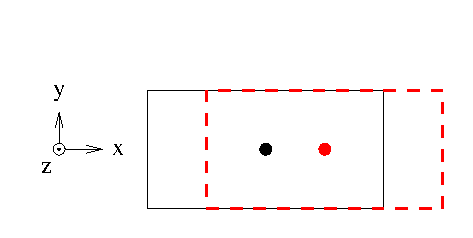
\includegraphics[width=\linewidth]{chamber_alignment/dof_x.pdf}
  \end{minipage} &
  \begin{minipage}{\linewidth}
    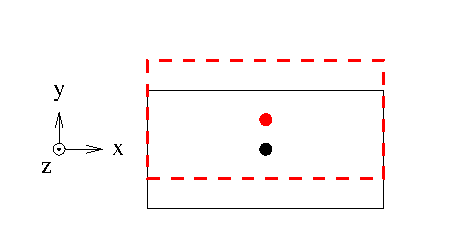
\includegraphics[width=\linewidth]{chamber_alignment/dof_y.pdf}
  \end{minipage} &
  \begin{minipage}{\linewidth}
    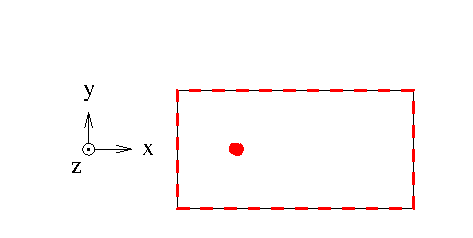
\includegraphics[width=\linewidth]{chamber_alignment/dof_z.pdf}
  \end{minipage} \\
  \begin{minipage}{\linewidth}
    \begin{center}
      $x$: offset in $r_x$
    \end{center}
  \end{minipage} &
  \begin{minipage}{\linewidth}
    \begin{center}
      $y$: offset in $r_y$
    \end{center}
  \end{minipage} &
  \begin{minipage}{\linewidth}
    \begin{center}
      $z$: sensitive only through angled tracks
    \end{center}
  \end{minipage} \\
  & & \\
  \begin{minipage}{\linewidth}
    \tiny
    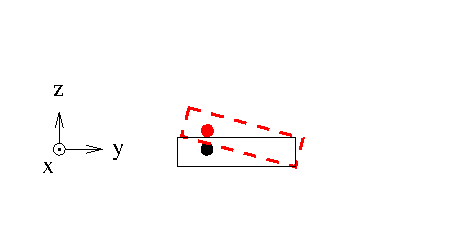
\includegraphics[width=\linewidth]{chamber_alignment/dof_phix.pdf} \\ \mbox{ }
  \end{minipage} &
  \begin{minipage}{\linewidth}
    \tiny
    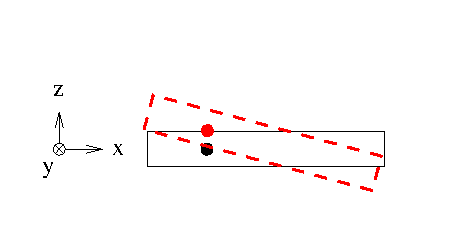
\includegraphics[width=\linewidth]{chamber_alignment/dof_phiy.pdf} \\ \mbox{ }
  \end{minipage} &
  \begin{minipage}{\linewidth}
    \tiny
    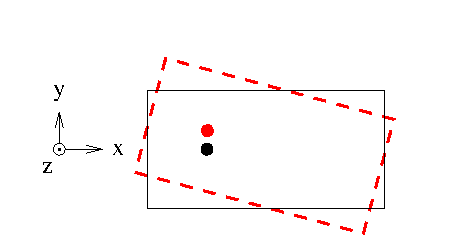
\includegraphics[width=\linewidth]{chamber_alignment/dof_phiz.pdf} \\ \mbox{ }
  \end{minipage} \\
  \begin{minipage}{\linewidth}
    \begin{center}
      $\phi_x$: $r_y$ linear in $y$ \\ \mbox{ }
    \end{center}
  \end{minipage} &
  \begin{minipage}{\linewidth}
    \begin{center}
      $\phi_y$: $r_x$ linear in $x$ \\ \mbox{ }
    \end{center}
  \end{minipage} &
  \begin{minipage}{\linewidth}
    \begin{center}
      $\phi_z$: $r_x$ linear in $y$ and \\ $r_y$ linear in $x$
    \end{center}
  \end{minipage} \\
  \begin{minipage}{\linewidth}
    \scriptsize
    \begin{center}
      (slope $\propto$ $1 - \cos\phi_x$)
    \end{center}
  \end{minipage} &
  \begin{minipage}{\linewidth}
    \scriptsize
    \begin{center}
      (slope $\propto$ $1 - \cos\phi_y$)
    \end{center}
  \end{minipage} &
  \begin{minipage}{\linewidth}
    \scriptsize
    \begin{center}
      (slope $\propto$ $\sin\phi_z$)
    \end{center}
  \end{minipage}
\end{tabular}
\end{center}

\caption{\label{profile_prediciton} The relationship between chamber
  degrees of freedom and trends in the residuals distriutions ($r_x$
  and $r_y$ versus local $x$ and $y$ coordinates of the track impact
  point).  Dependence on $z$, $\phi_x$, and $\phi_y$ is weak.}
\end{figure}


\begin{figure}
  \begin{center}

    \begin{tabular}{p{0.3\linewidth} p{0.3\linewidth} p{0.3\linewidth}}
      \begin{minipage}{\linewidth}
	\begin{center} \mbox{\hspace{0.4 cm}} Ideal chamber positions \end{center}
      \end{minipage} &
      \begin{minipage}{\linewidth}
	\begin{center} \mbox{\hspace{0.4 cm}} Offset 1~cm in $x$ \end{center}
      \end{minipage} &
      \begin{minipage}{\linewidth}
	\begin{center} \mbox{\hspace{0.4 cm}} Rotated 1~mrad in $\phi_z$ \end{center}
      \end{minipage} \\
      \begin{minipage}{\linewidth}
	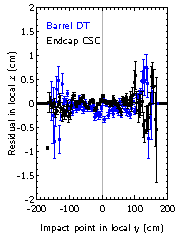
\includegraphics[width=\linewidth]{chamber_alignment/init_xresid_vs_y.pdf}
      \end{minipage} &
      \begin{minipage}{\linewidth}
	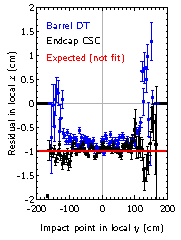
\includegraphics[width=\linewidth]{chamber_alignment/x_xresid_vs_y.pdf}
      \end{minipage} &
      \begin{minipage}{\linewidth}
	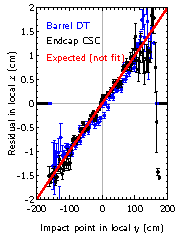
\includegraphics[width=\linewidth]{chamber_alignment/phiz_xresid_vs_y.pdf}
      \end{minipage}
    \end{tabular}
  \end{center}

\caption{\label{profile_demonstration} Demonstration of the trends
  presented in Figure~\ref{profile_prediciton} with coherently
  misaligned chambers.}
\end{figure}



\pagebreak

\section{-------- Old organization below this line; not necessarily
  consistent with new organization --------}

\section{Nominal procedure}

We will first describe the nominal alignment procedure.  This is the
procedure by which routine alignment corrections are obtained, and the
point of comparison for systematics studies.

\subsection{Wheel and disk granularity}

The first step in the procedure, as explained above, is to align the
largest level of granularity: wheels in the barrel and disks in the
endcap.

\subsection{Chamber-by-chamber}

default, standard of comparison

10 pb$^{-1}$ of high $p_T$ tracks (from $Z$'s and $W$'s)

number of hits cuts on tracks, pull cut on hits

Initial misalignment: the Muon10InvPbScenario with residual layer
misalignments (to be determined from layer alignment studies)

chamber-by-chamber (CSC and DT) x, phiy, phiz float?  can we relax
this, letting y and phix float, too?  Not for DT station 4, of course...

globalMuon APE scheme: starts large, descends rapidly, converges
in a few iterations

standAloneMuon APE scheme: less steep, but relevant

\section{Accuracy and Precision}

output alignment parameter uncertainties (are they broken?  why
are they $\sim$4 times too big?): do they scale with residual
misalignment?

if not, is there any other way to identify chambers with poor
convergence?  do they have fewer hits?

\section{Performance issues}

How does this scale with number of tracks (convert to pb$^{-1}$ of $W$,
$Z$, and if possible, a generic muon sample with a cut)

How much computer time does this take?  (per iteration, and how
many iterations are necessary?)

\section{Special alignments}

\subsection{Quick disk alignment}

how much data do we need to do this if the
chambers and layers are also misaligned?  (With ideal chambers,
it's very quick! {\tt :)}

MC and MTCC (compare with known x = 7 mm, y = 1 mm in MTCC phase II)

\subsection{CSC Layer alignments}

what is the nominal procedure, what degrees
of freedom can we align, and how much data do we need to do it?

MC and MTCC

this will probably include Karoly's work: his plots with our results overlaid

\section{Beam halo alignment of CSC layers}

will we have this before data-taking?

New information from Karoly: no problem for inner ring, outer ring may
have 0.8 million muons, though heavily emphasizing the inner radius part

\section{Systematics studies}

\subsection{Dependence on tracker alignment}

How does the globalMuon strategy depend on tracker alignment?
(Initial studies suggest that the dependence is {\it very} weak.  Is
there anything wrong with my studies?)

New information: it looks like my procedure is working.  Dependence on
tracker alignment is probably {\it very weak!}  I need to pull this
together into a coherent story, with plots.

\subsection{Dependence on momentum}

How does resolution depend on the momentum of the input tracks?
Use $J/\psi$s to do an alignment if you have enough; otherwise, just
compare width of the residuals distributions.

\subsection{Dependence on fitting parameters}

What happens if we use different sets of fitting parameters?  I
don't see much difference yet, but I haven't tried dropping "y"
degrees of freedom.

\subsection{Correlation between alignment and calibration}

How well does alignment fare if we have a miscalibrated detector?

\subsection{``Dependence on tracking algorithm''}

\subsubsection{Uncertainty in material distribution}
Change the distribution of material in track-fitting but not
in SimHit generation to simulate incorrect material
description

\subsubsection{Uncertainty in magnetic field}

Same for magnetic field modeling

\subsubsection{Dependence on track charge}

How does alignment differ between positive and negative
tracks?  Can we cancel the effect by requiring equal
populations?

\subsubsection{Depdence on the actual algorithm used in tracking}

If I'm very adventurous, I may try plugging in different
tracking algorithms.  I don't know how easy that is.

\subsection{Background studies}

Align with realistic backgrounds from CSA07

What are the optimized track quality cuts?

\section{Conclusion}

It works very, very, very well.

\end{document}
